\section{Evaluation}
\label{sec:evaluation}

In this section, we present an experimental evaluation of \projecttitle based on the implementation described in  \secref{implementation}. Our evaluation answers the following questions.

\begin{itemize}
\item What overheads does \projecttitle impose for recording data provenance of multithreaded executions? ($\S$~\ref{subsec:overheads})
\item How do these overheads scale with increases in the size of input data and computation size? ($\S$~\ref{subsec:scale-overheads})
\item What are the sources for the provenance overheads? ($\S$~\ref{subsec:quantify-overheads})
\end{itemize}



\subsection{Experimental Setup}
We first describe the experimental setup used for the evaluation.

\myparagraph{Experimental platform} We used an Intel Xeon processor based
multicore architecture as our host machine for our evaluation. The
host system consists of 8 cores (16 threads) of Intel(R) Xeon(R) CPU Processor D-1540
(12M Cache, 2.00 GHz) and 32 GB of DRAM main memory. The host
machine is running Linux with kernel 4.2.0 in 64-bit mode.


\myparagraph{Applications and dataset}  We evaluated \projecttitle with applications from two multithreaded benchmark suites: Phoenix 2.0 \cite{phoenix} and PARSEC 3.0 \cite{parsec}. Table~\ref{tab:apps} lists the applications used for the evaluation along with the input data and benchmark parameters.





\myparagraph{Metrics: Time and Work}  We consider two types of measures to report the performance metrics: {\em time} and {\em work}. In a nutshell, time measurements reflect the end user perceived latency, whereas work measurements assess the overall resource (CPU) utilization.  More specifically,  time refers to the end-to-end computation time for the multithreaded applications. Work refers to the total computation performed by all threads, and it is measured as the cumulative CPU time for all threads. To measure work, we used the CPU accounting controller in cgroups to account the CPU usage of all threads.

\myparagraph{Measurements} All applications were compiled using GCC 5.2.1 compiler with -$o3$ optimization flag. For all performance measurements, we report the average over 10 runs with minimum and maximum values discarded.


\begin{figure}[t]
\centering
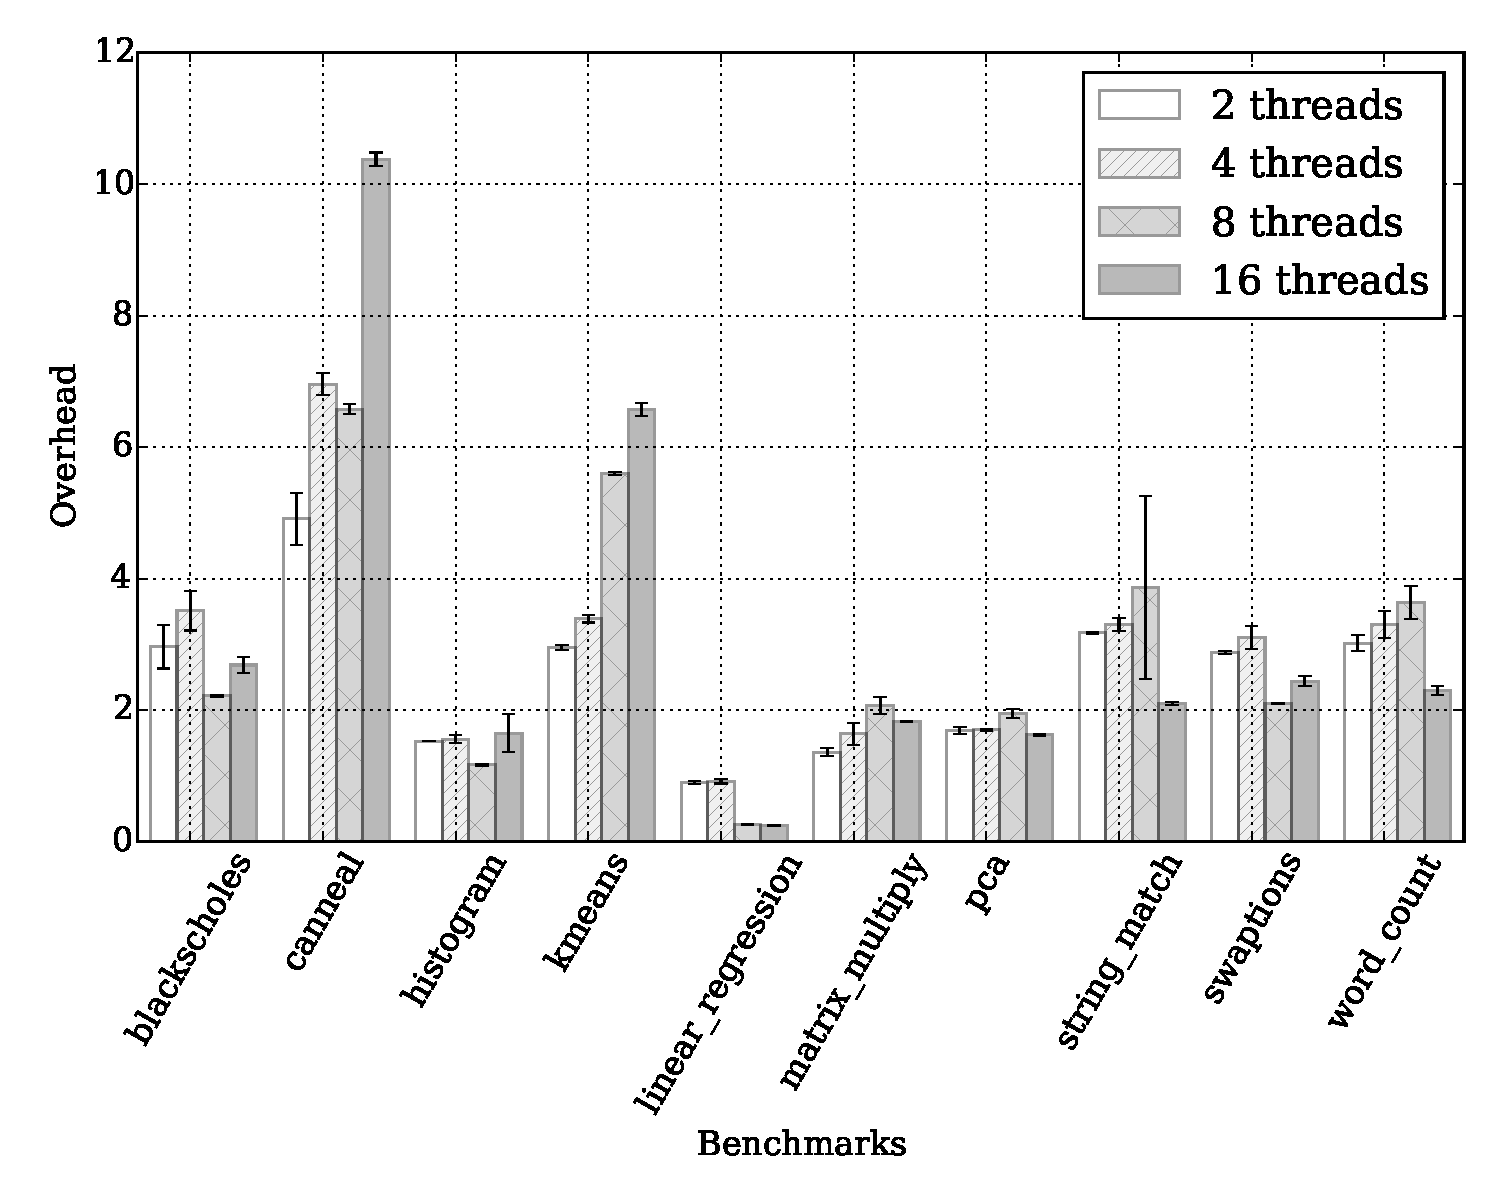
\includegraphics[scale=0.46]{figure/benchmarks/times-inspector.pdf}
\caption{Performance overhead  over native execution with increasing number of threads.}
\label{fig:overheads}
\end{figure}


\begin{figure}[t]
\centering
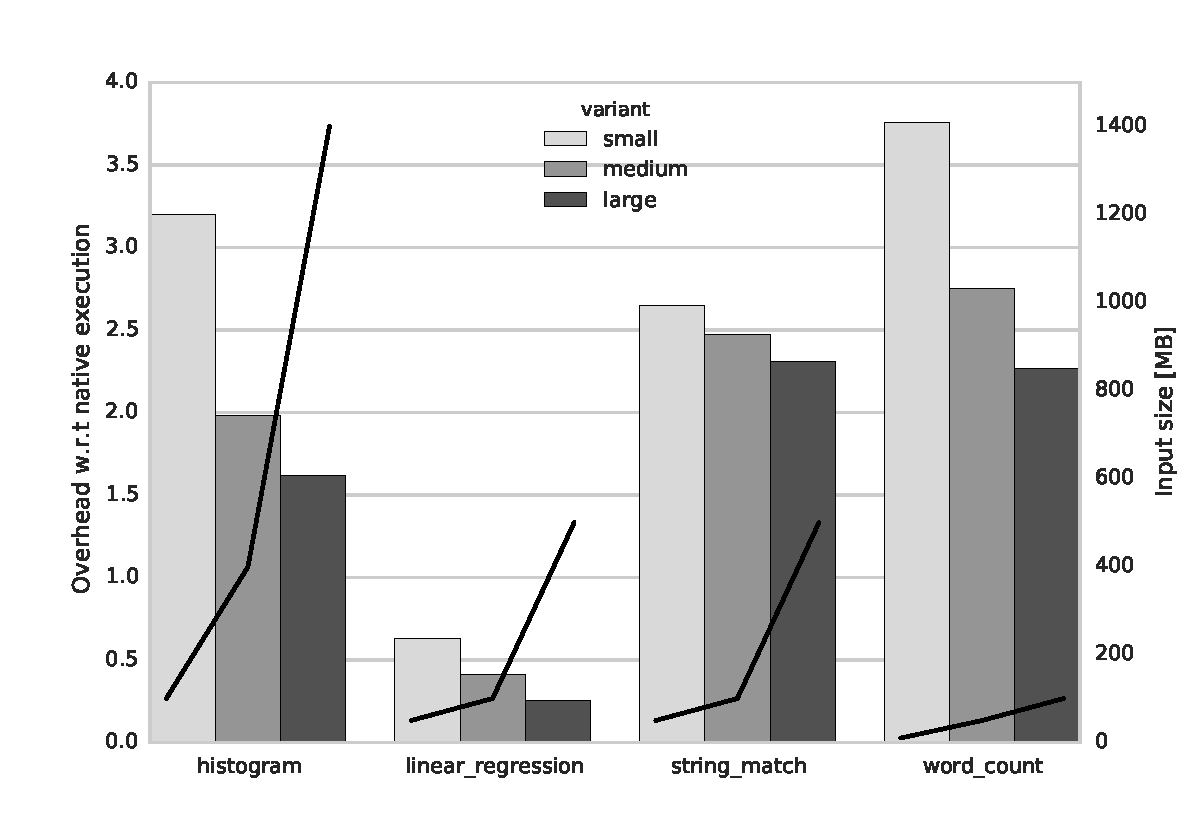
\includegraphics[scale=0.3]{figure/benchmarks/worksize-times-xy.pdf}
\caption{Scalability of overheads with increase in the input data sizes with $16$ threads. }
\label{fig:data-size-overheads}
\end{figure}



\begin{figure}[t]
\centering
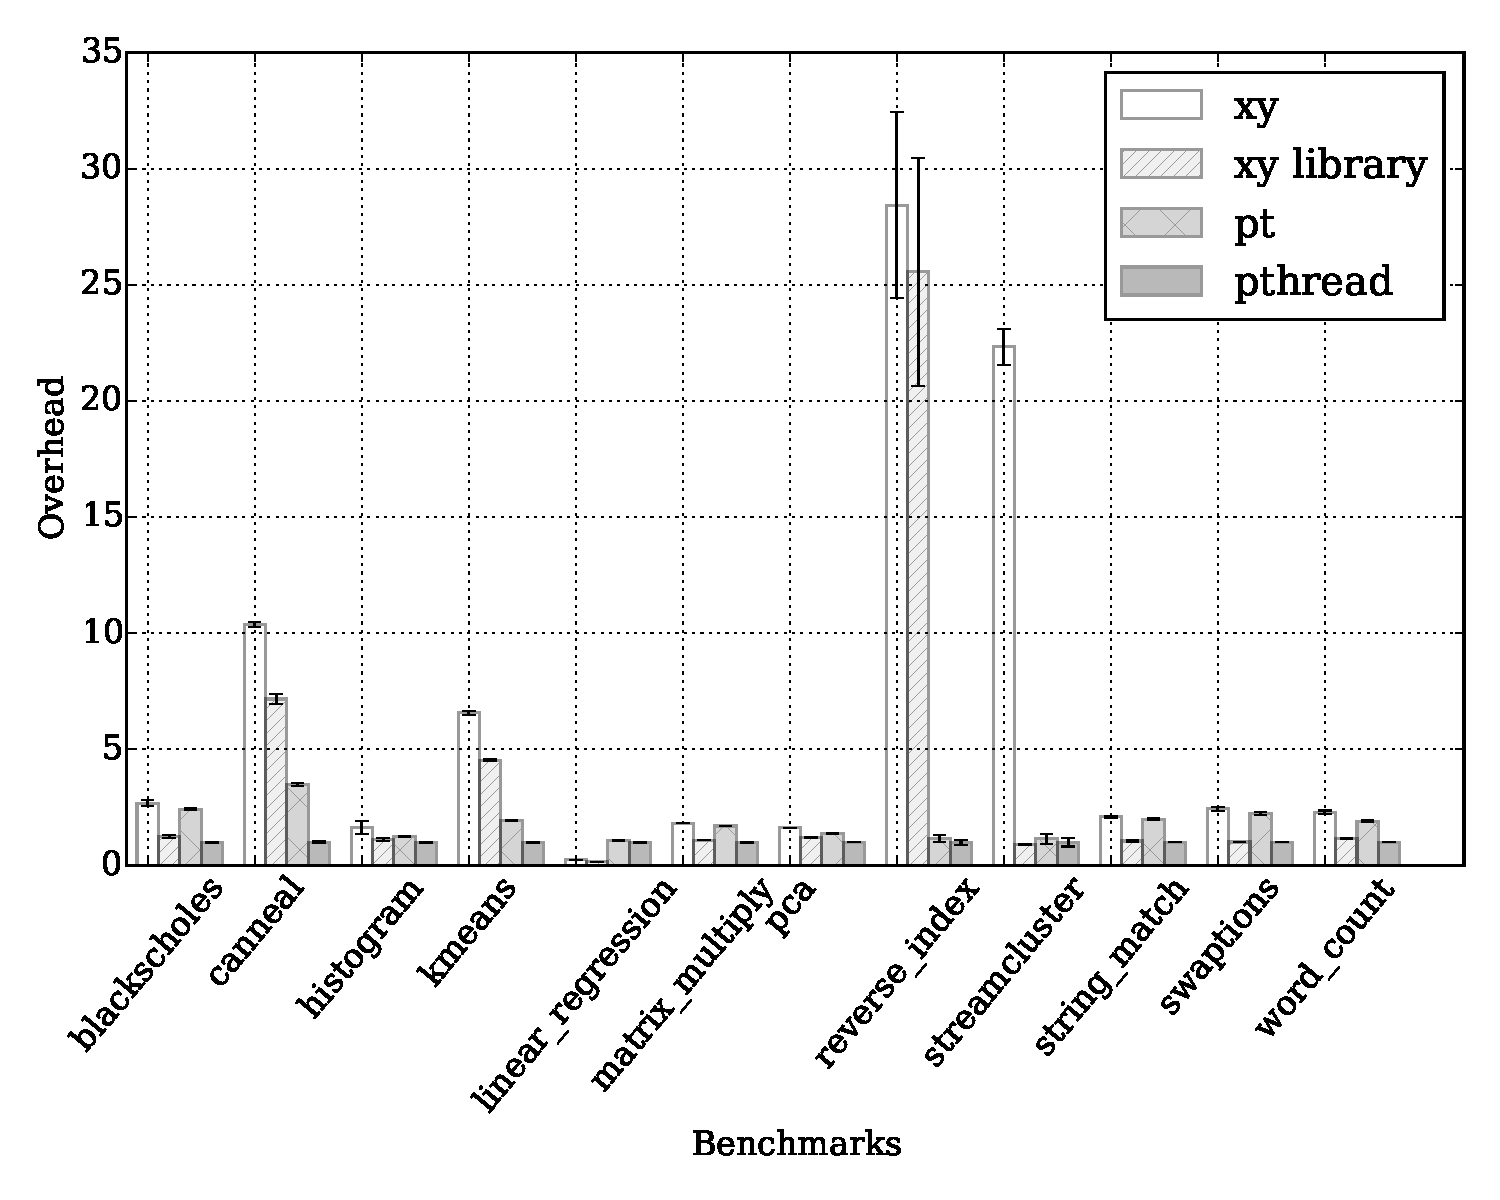
\includegraphics[scale=0.43]{figure/benchmarks/times-16-threads.pdf}
\caption{Performance overhead breakdown with $16$ threads --- except for streamcluster, where overhead for 15 threads is shown}
\label{fig:overheads-breakdown}
\end{figure}


\if 0
\begin{figure}[h]
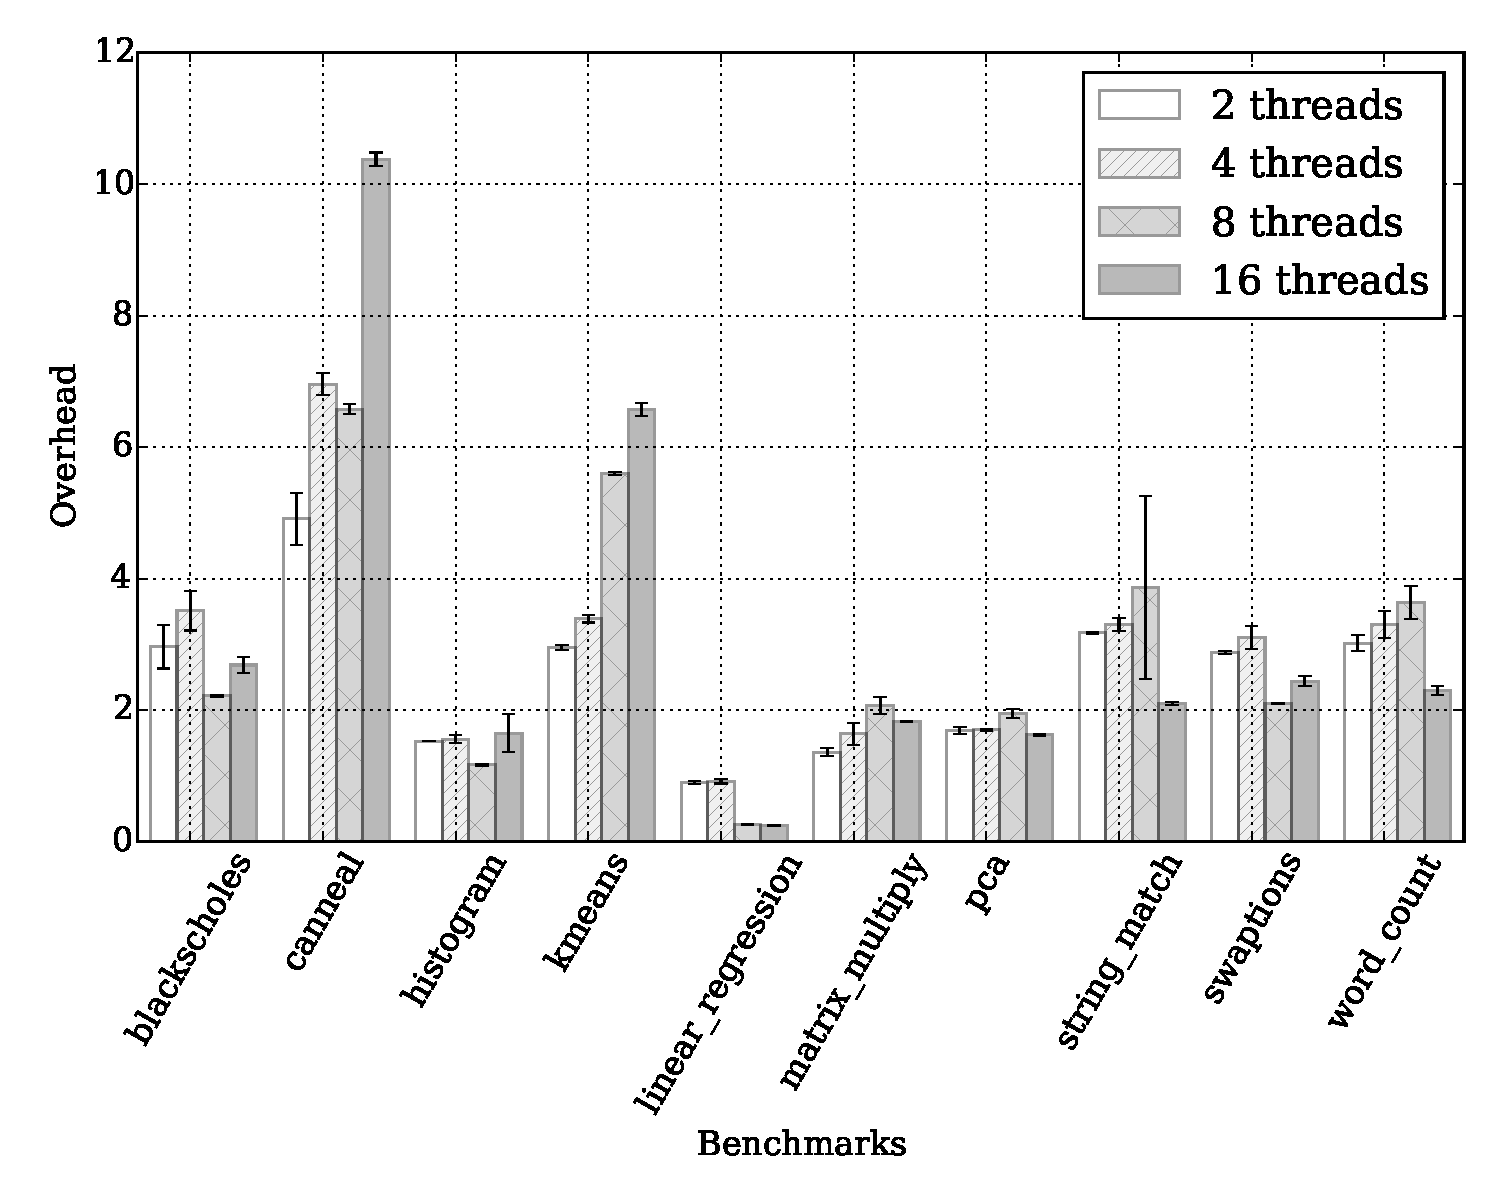
\includegraphics[width=8cm]{figure/benchmarks/times-inspector.pdf}
\end{figure}

\begin{figure}[h]
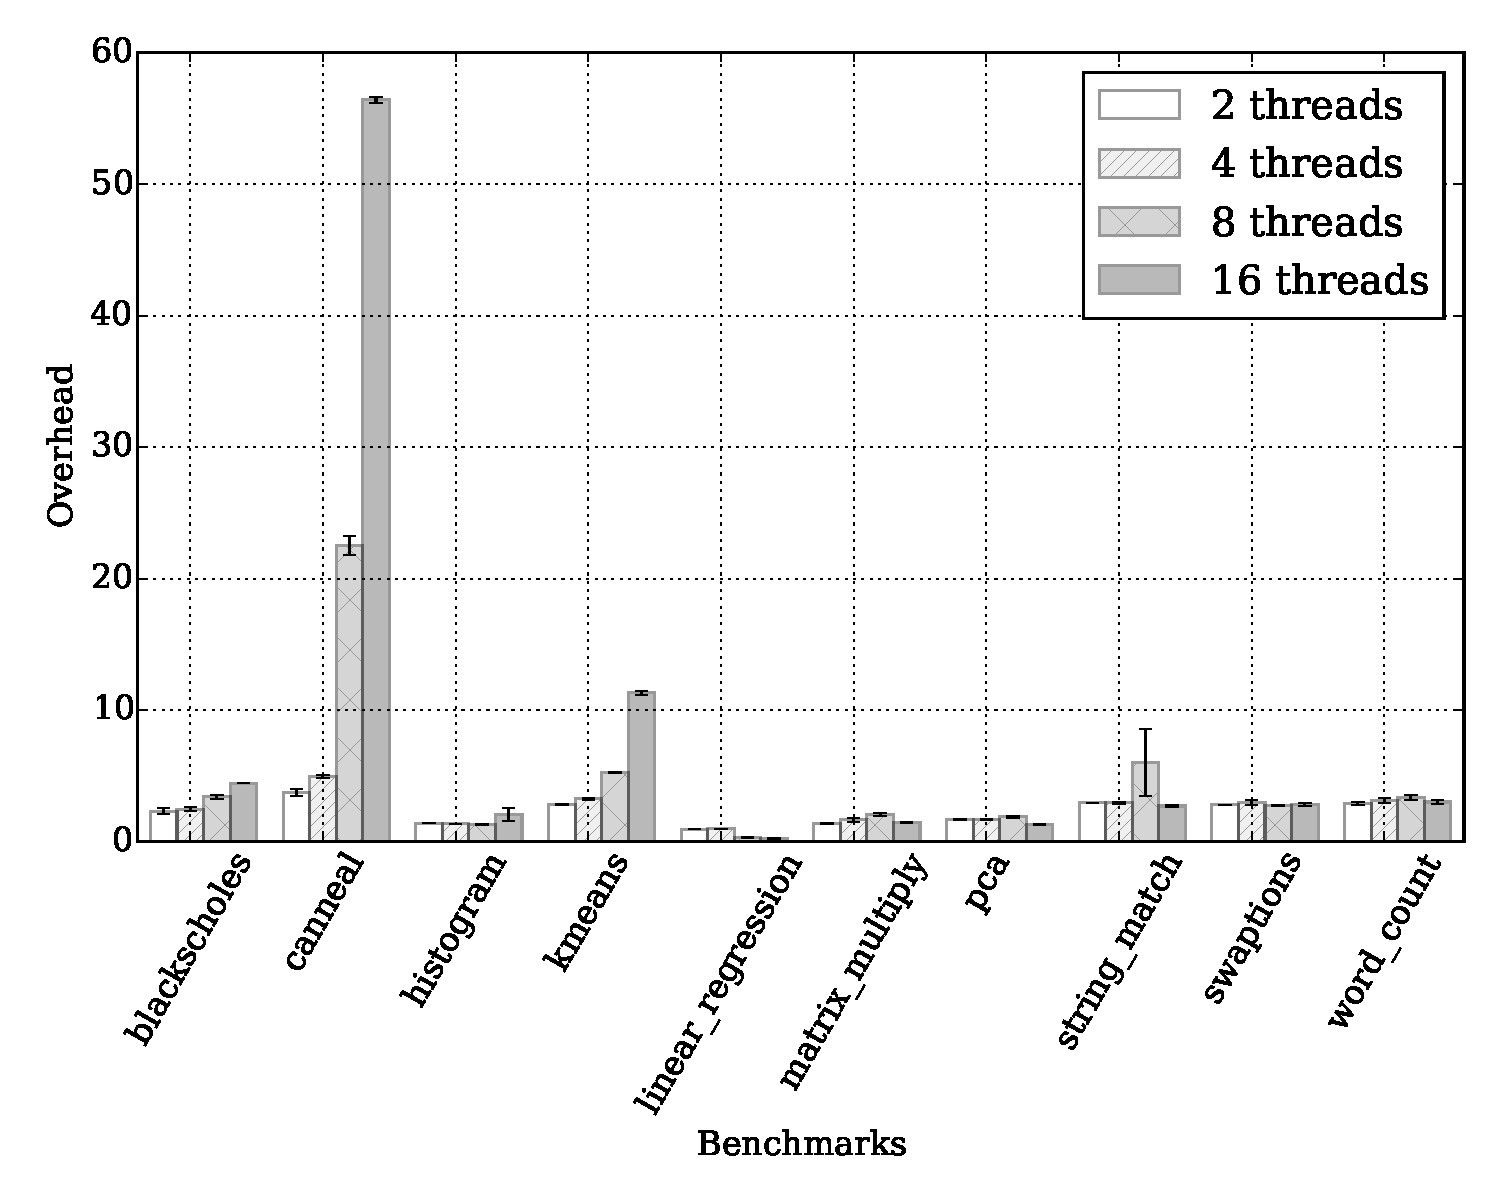
\includegraphics[width=8cm]{figure/benchmarks/cpu-cycles-inspector.pdf}
\end{figure}

\begin{figure}[h]
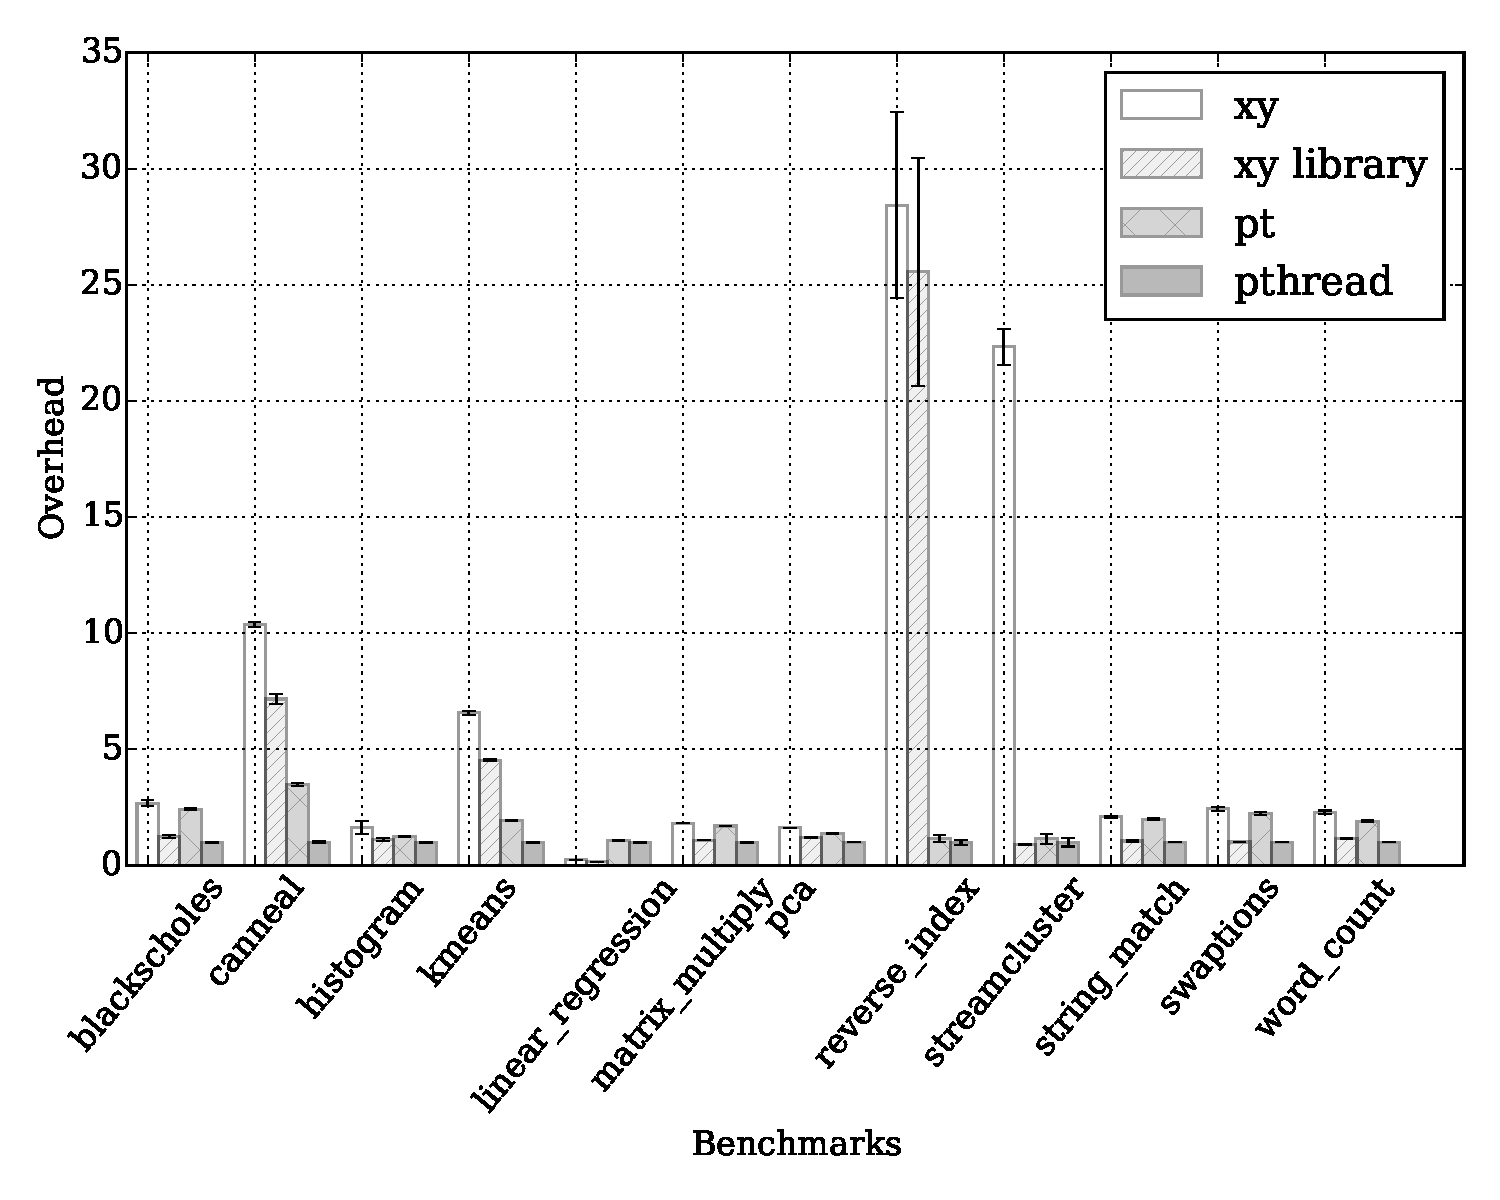
\includegraphics[width=8cm]{figure/benchmarks/times-16-threads.pdf}
\end{figure}

\begin{figure}[h]
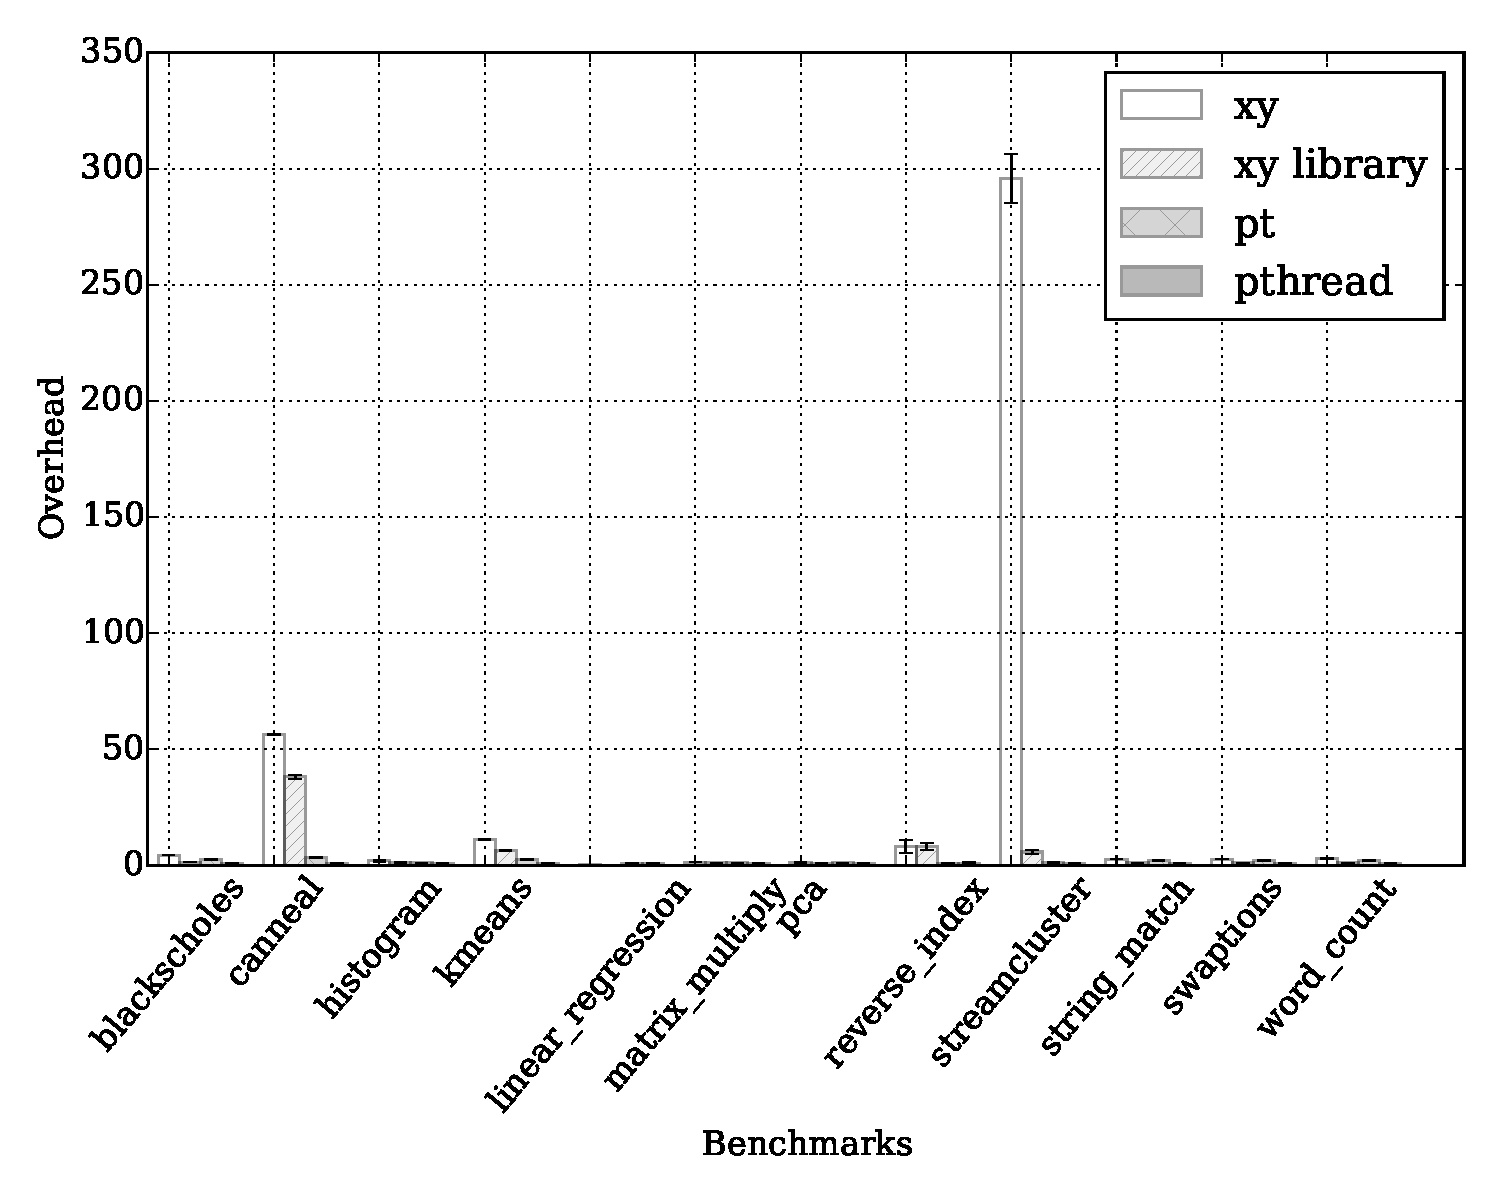
\includegraphics[width=8cm]{figure/benchmarks/cpu-cycles-16-threads.pdf}
\end{figure}

\begin{figure}[h]
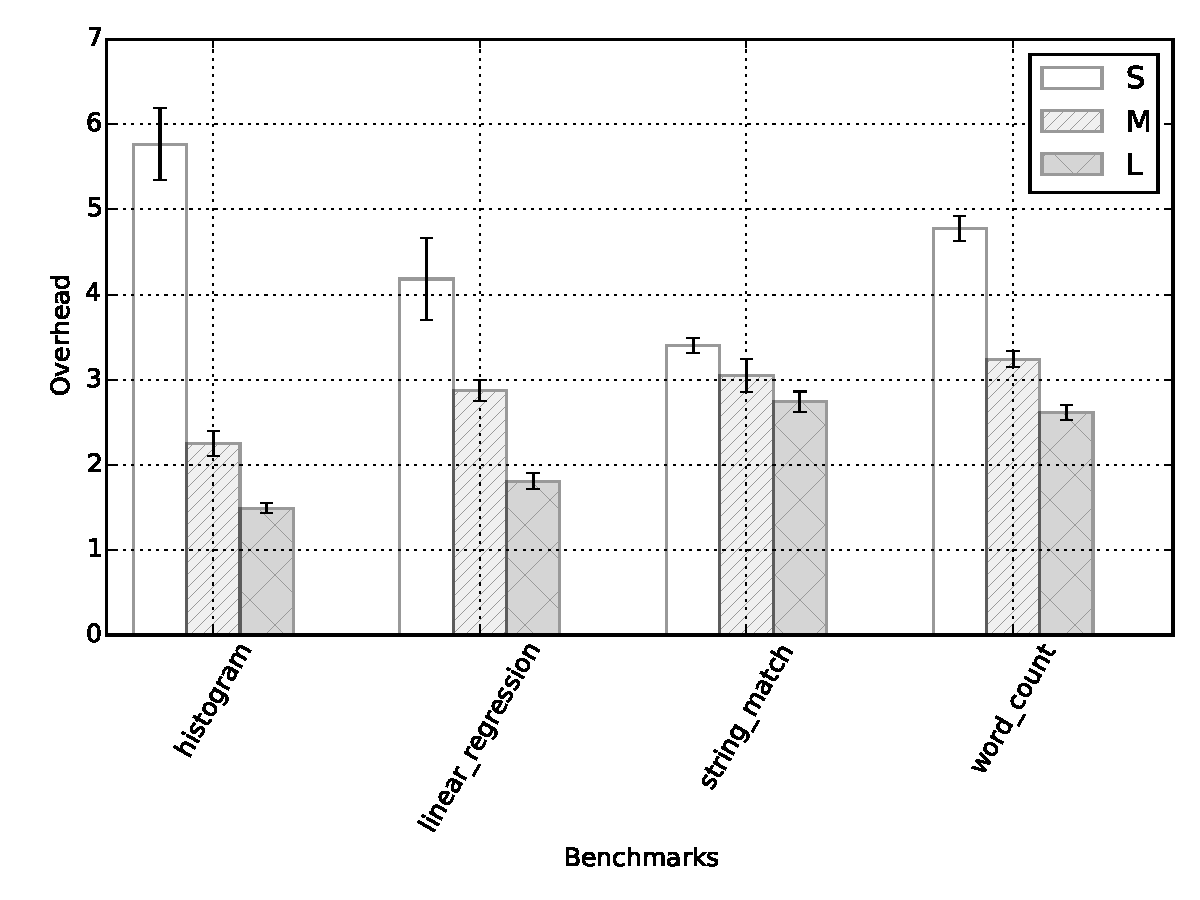
\includegraphics[width=8cm]{figure/benchmarks/worksize-times-inspector.pdf}
\end{figure}
\fi 
%
%\myparagraph{Performance metrics: Work and Time}  For each run, we consider two types of measures: \emph{work} and
% {\em time}. Work refers to the total amount of
%computation performed by all threads and is measured as the total
%run-time of all threads. Time refers to the amount of (end-to-end)
%run-time to complete the parallel computation. Both metrics are important
%and complementary: time measurements reflect the end user perceived latency,
%whereas work measurements assess the overall resource (CPU) utilization.

\subsection{Provenance Overheads}

\myparagraph{Overheads}

\myparagraph{Breakdown of overheads}

\subsection{\projecttitle Scalability}

\myparagraph{Overheads w.r.t. input size}

\myparagraph{Overheads w.r.t. computation size}


\subsection{Sources of Overheads}

% -*- root: ../main.tex -*-

% Dmitrii: couldn't find a way to make dynamic multicolumn with csvreader, so just copy-pasted result here from tables/data/avxbenches-stats.csv

\begin{table*}[t]
\footnotesize
\centering

\begin{tabular}{l | r r r || l | r r r}
%[-8pt]
\bfseries Bench & \bfseries ILP & \bfseries AVX & \bfseries inc & \bfseries Bench & \bfseries ILP & \bfseries AVX & \bfseries inc \\
\hline                    
\hline
hist      & 2.13  & 60.1  &  8.56 & black    & 1.77 & 76.6 & 1.70 \\
km        & 2.58  & 73.2  &  6.37 & dedup    & 1.75 & 60.7 & 4.64 \\
linreg    & 1.70  & 55.0  & 10.49 & ferret   & 1.81 & 67.2 & 4.32 \\
mmul      & 0.96  & 77.2  &  4.47 & fluid    & 1.54 & 75.8 & 2.43 \\
pca       & 2.28  & 77.4  &  6.82 & scluster & 1.22 & 77.1 & 3.77 \\
smatch    & 3.26  & 52.1  & 32.72 & swap     & 2.06 & 70.5 & 3.50 \\
wc        & 2.24  & 70.9  &  6.14 & x264     & 2.00 & 59.3 & 3.26 \\
\hline
\end{tabular}


\caption{Runtime statistics for versions of benchmarks with 16 threads: ILP (in instr/cycle), fraction of AVX instructions (in percents), and increase in number of all instructions w.r.t. native.}
\label{tab:apps}

\end{table*}





